\documentclass{article}

% formatting
\usepackage[utf8]{inputenc} % allow utf-8 input
\usepackage[T1]{fontenc} % use 8-bit T1 fonts  (allows for direct use of ö,ü,etc.)

% math typesetting
\usepackage{amsmath}
\usepackage{amsfonts}

% color
\usepackage{color}
\usepackage{xcolor}

% layout
\usepackage{layout}
\usepackage{lipsum}

% cross-referencing and hyperlinks
\usepackage{hyperref}
\usepackage{url}
\usepackage{doi}

% figures
\usepackage{graphicx}

% tables
\usepackage{booktabs}
\usepackage{multirow}
\usepackage{caption} 
\usepackage{float}

% enumeration
\usepackage{enumitem}

% embedding pages
\usepackage{pdfpages}

% multi-line comments
\usepackage{comment}

% footnotes
\usepackage{footnote}

\usepackage{subfig}
\usepackage{cleveref}

\usepackage[
    backend=biber,
    style=authoryear-comp
]{biblatex}
\addbibresource{references.bib}

%%%%%%%%%%%%%%%%%%%%%%%%%%%%%%%%%%%%%%%%%%%%%%%%%%%%%%%%%%%%%%%%%%%%%

% document metadata
\title{Proposal for a Summer Academy of the Swiss Study Foundation}
\author{Michael Weinold, Philippe Schultheiss et al.}
\date{2023}

%%%%%%%%%%%%%%%%%%%%%%%%%%%%%%%%%%%%%%%%%%%%%%%%%%%%%%%%%%%%%%%%%%%%%

\begin{document}

\maketitle

\tableofcontents

\section{Introduction}

\begin{figure}[]
    \centering
    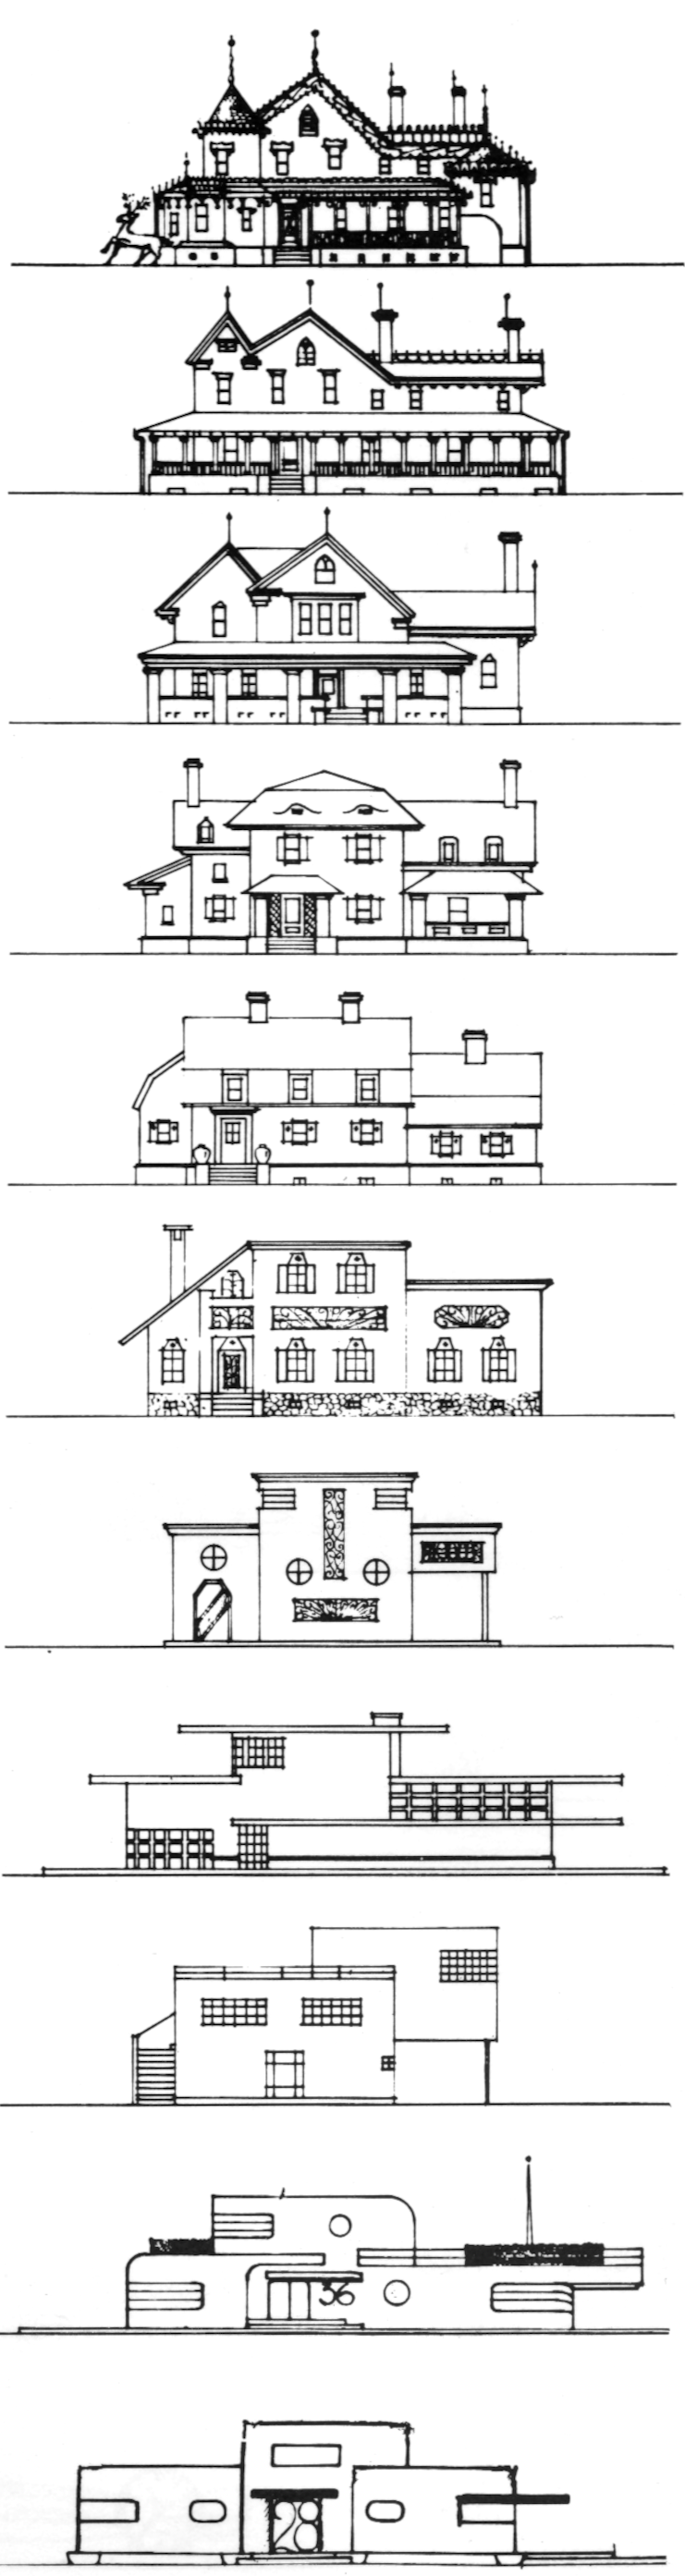
\includegraphics[height=\textheight]{./figures/loewy_architecture.png}
    \caption{
        Some text here. Source: "Design Evolution 1930", \cite{loewy_industrial_1979}
    }
    \label{fig:combined}
\end{figure}

\section{Scope of the Discussion}

Modern architecture is always ugly. Nonetheless, we limit our discussion to buildings of a representative nature. We exclude housing (eg. apartment complexes) to avoid:

\section{Scattered Thoughts}

Architects have been publicly calling for the public to be re-educated to appreciate their brutalist/modernist designs. (eg. the architects that build the Triemli Tower).

Some potential pathways to decarbonizing the economy are difficult for technical and political reasons. This includes "flying less", "reducing personal mobility", etc.
However, some aspects should be really simple: "don't design houses for a 50 year lifetime"

\section{Sustainability}

\section{Aesthetics}

\textit{"[Architecture] (...) is the most overweening of the arts, and the one that least lets us alone. A gallery we can't walk out of, a book we can't close, an art we can't even turn our back on because it is there facing us on the other side of the street as well (...)} - British poet Blake Morrison in "Lords of glass, steel and concrete" \cite{morrison_lords_1982}

\section{Connecting Aesthetics and Sustainability}



Studies show that 

\begin{figure}
    \centering
    \subfloat{{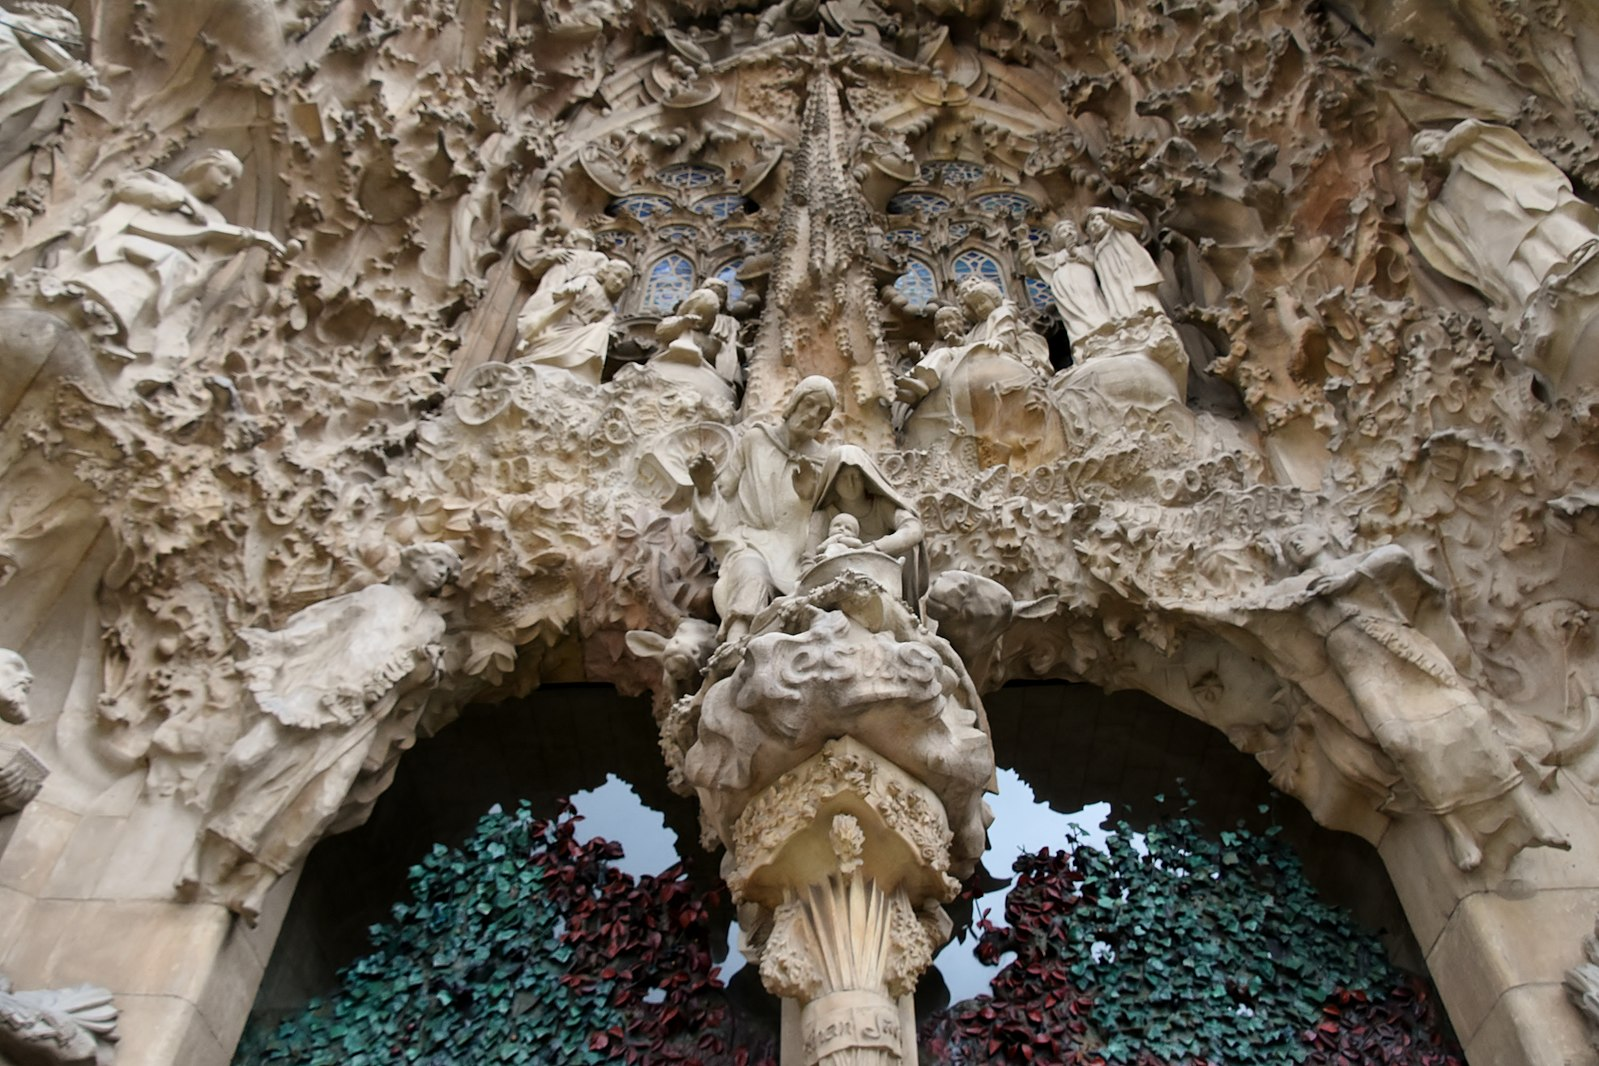
\includegraphics[height=4cm]{figures/sagrada_facade.jpg} }}
    \subfloat{{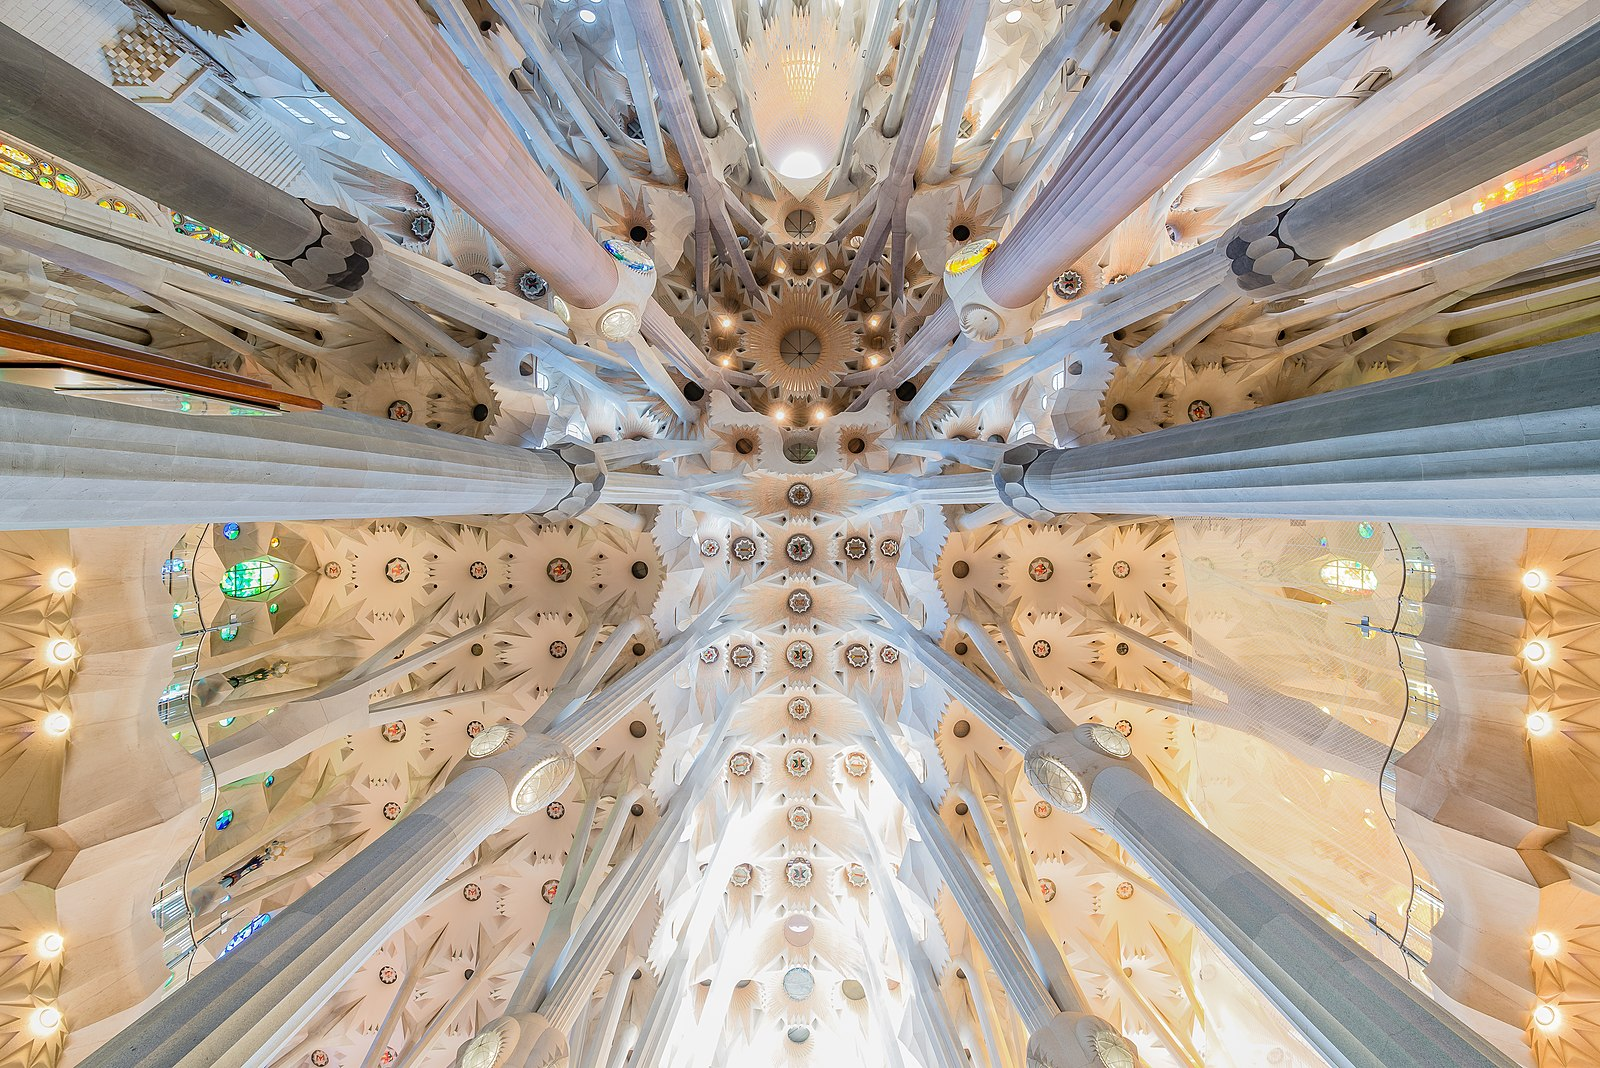
\includegraphics[height=4cm]{figures/sagrada_interior.jpg} }}
    \caption{Gothic Revival, Art Nouveau and Modernista catholic church "Sagrada Familia" (en.: "Holy Family") in Barcelona, Spain, designed by Antoni Gaudí from 1883 until his death in 1926. Left: Detail of the nativity façade with XXXX. Right: Wide-angle view of the   Image sources from left to right: Outside view \cite{mortel_sagrada_2016} and inside view \cite{wikimedia_commons_user_t_meltzer_sagrada_2014}.}
    \label{fig:kunstformen}
\end{figure}

\begin{figure}
    \centering
    \subfloat{{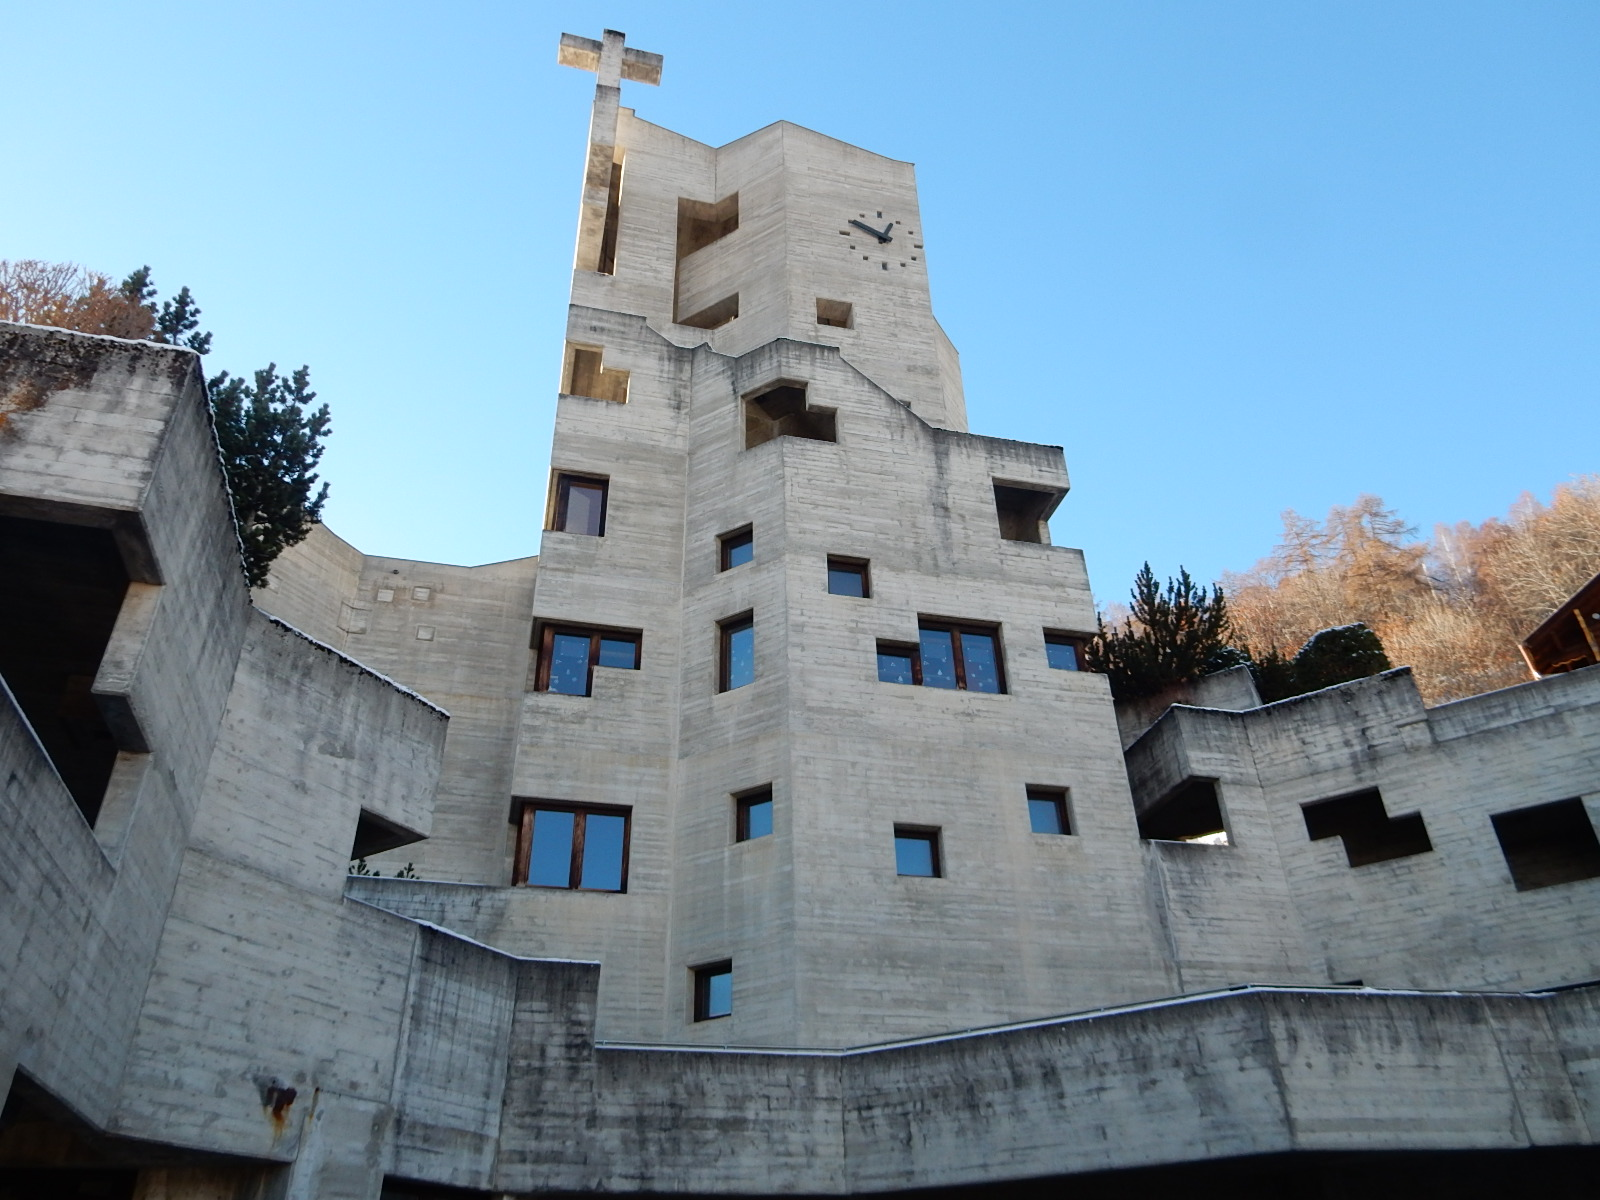
\includegraphics[height=4.5cm]{figures/hérémence_1.jpg} }}
    \subfloat{{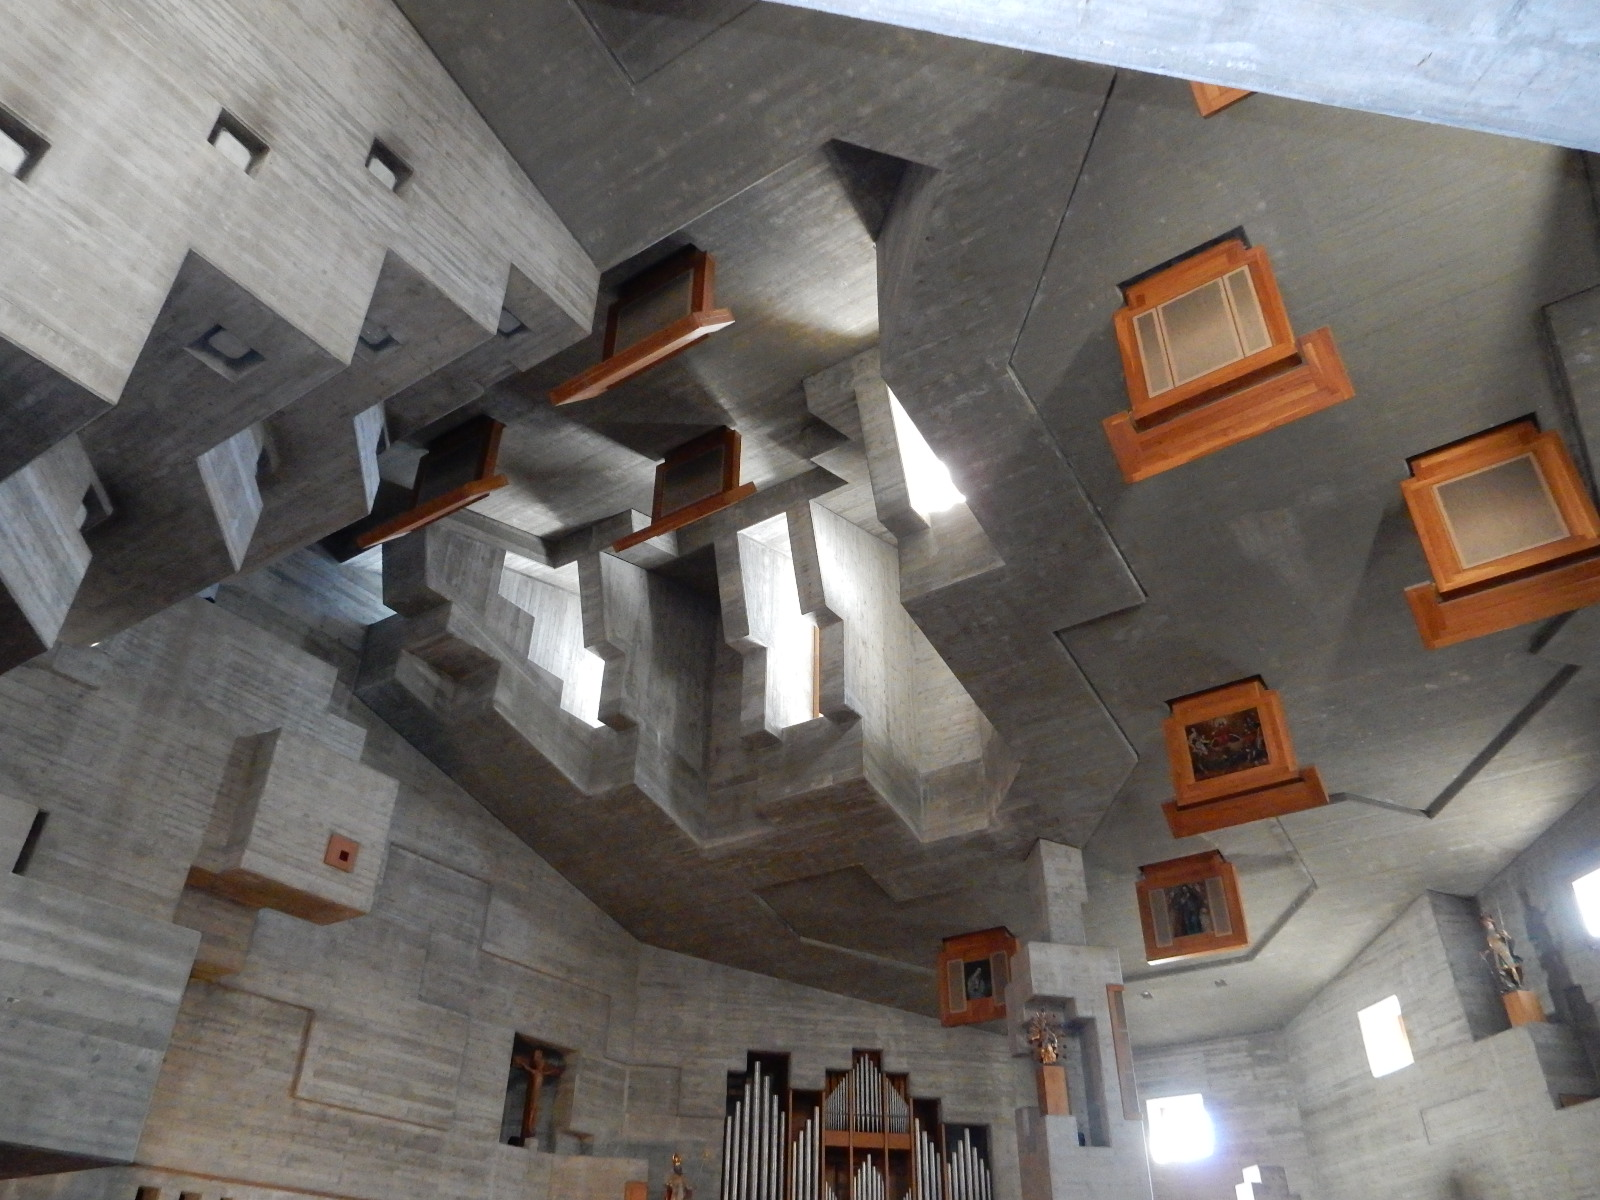
\includegraphics[height=4.5cm]{figures/hérémence_2.jpg} }}
    \caption{Brutalist-style catholic church "St. Nicolas" in the Swiss mountain village of Hérémence, designed by Walter Maria Förderer in 1967. Image sources from left to right: Outside view \cite{bissegger_eglise_2018-1} and inside view \cite{bissegger_eglise_2018}.}
    \label{fig:kunstformen}
\end{figure}

\newpage

\begin{figure}
    \centering
    \subfloat{{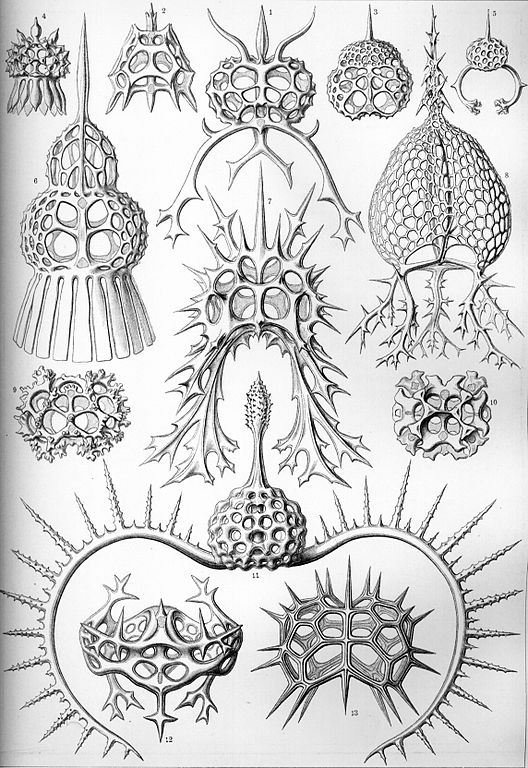
\includegraphics[height=5.5cm]{figures/Spyroidea.jpg} }}
    \subfloat{{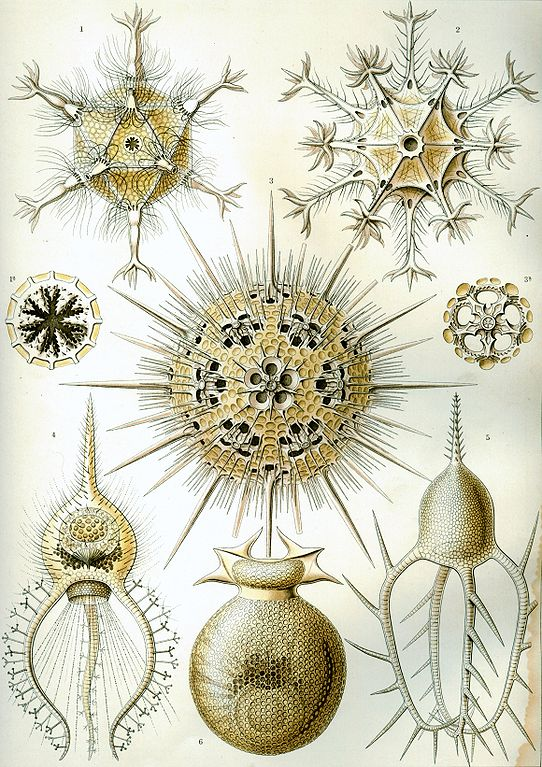
\includegraphics[height=5.5cm]{figures/Phaeodaria.jpg} }}
    \subfloat{{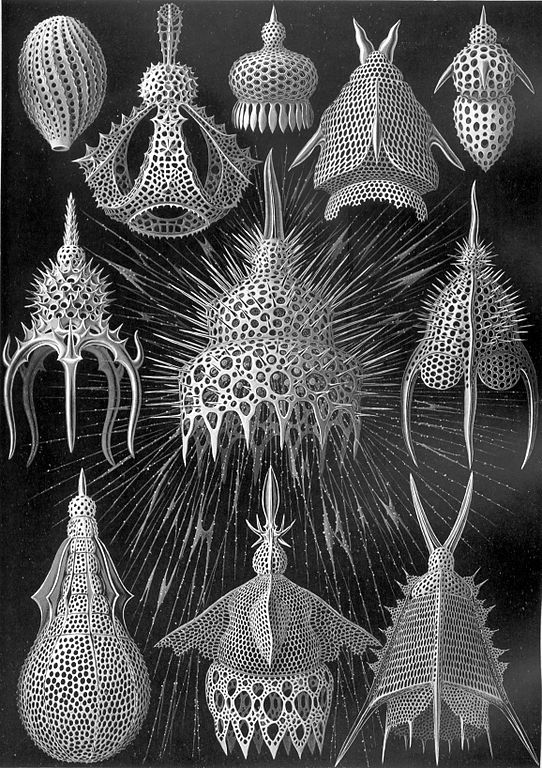
\includegraphics[height=5.5cm]{figures/Cyrtoidea.jpg} }}
    \caption{Selection of drawings from Ernst Haeckel's \textit{"Kunstformen der Natur" (en.: "Art Forms in Nature")} \cite{haeckel_kunstformen_2012}. According to Rene Binet, drawings like these served as inspiration for his monumental arch \cite[Sec. "Haeckel und der Jugendstil"]{willmann_haeckel_2019}, which is depicted in \cref{fig:arch}. Image sources from left to right: Spyroidea \cite{haeckel_kunstformen_1904}, Phaeodaria \cite{haeckel_kunstformen_1904} and Cyrtoidea \cite{haeckel_kunstformen_1904-2} by Ernst Haeckel.}
    \label{fig:kunstformen}
\end{figure}

\begin{figure}
    \centering
    \subfloat{{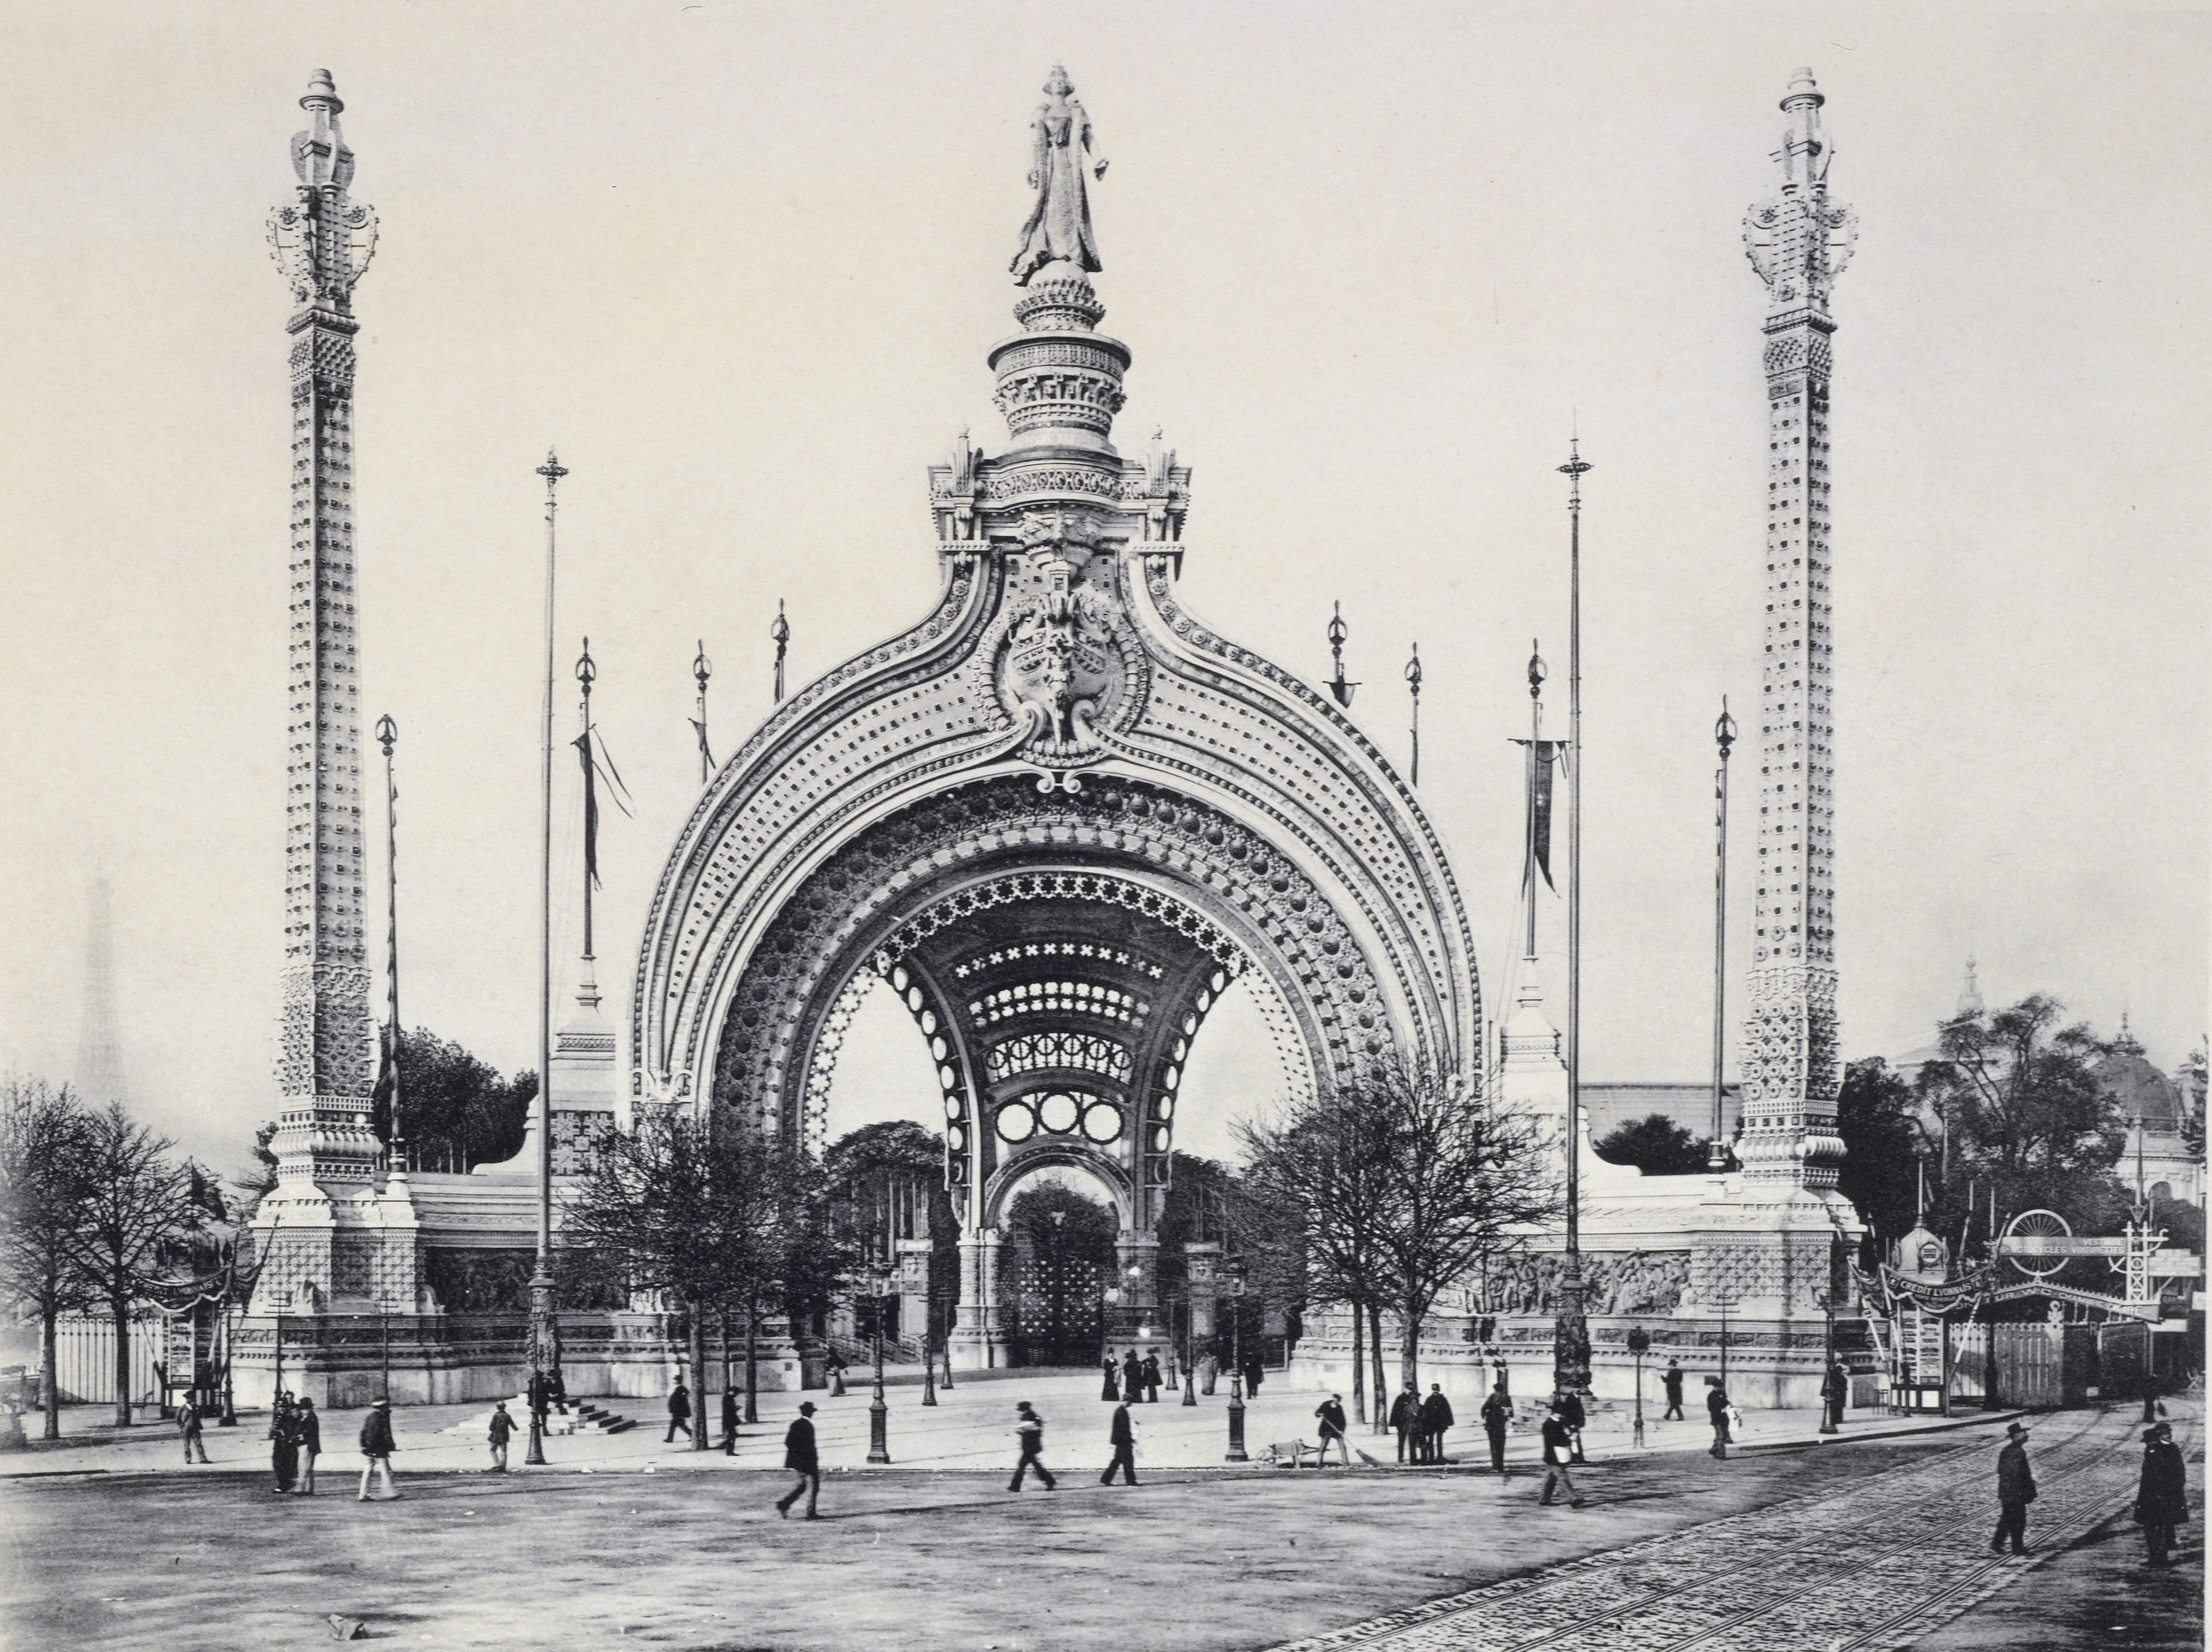
\includegraphics[height=4cm]{figures/porte_photograph.jpg} }}
    \subfloat{{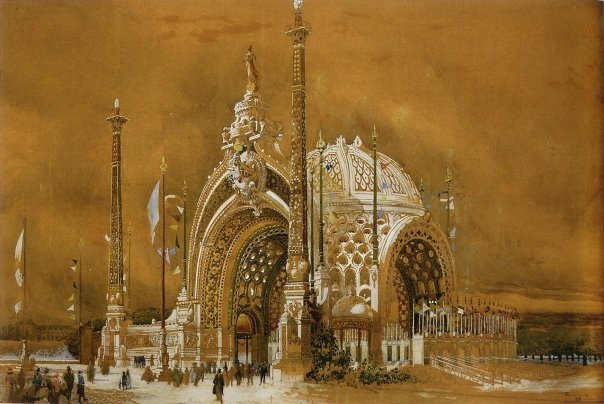
\includegraphics[height=4cm]{figures/porte_watercolor.jpg} }}
    \caption{Two renderings of the \textit{"Porte Binet"}, a monumental gate designed by Rene Binet for the 1900 Paris Exposition. Image sources: Photograph by Larger \cite{louis_porte_1900} and watercolor on paper by Binet \cite{binet_projet_1898}.}
    \label{fig:arch}
\end{figure}

\clearpage
\printbibliography

\end{document}
